\chapter{Introducci\'on}\label{ch:introduccion}

\epigraph{Mathematics knows no races
	or geographic boundaries;
	for mathematics,
	the cultural world
	is one country.}{"David Hilbert"}

\section{Introduction}


La promesa de la inteligencia artificial ha sido un tema de inter\'es p\'ublico y privado durante d\'ecadas. A partir de la d\'ecada de 1950, hubo grandes esperanzas de que las t\'ecnicas cl\'asicas de inteligencia artificial basadas en l\'ogica, representaci\'on del conocimiento, razonamiento y planificaci\'on dar\'ia lugar a un software revolucionario que podr\'ia, entre otras cosas, comprender el lenguaje, controlar robots y proporcionar asesoramiento experto. Aunque los avances basados en tales t\'ecnicas pueden estar al alcance en el futuro, muchos comenzaron a dudar de estos enfoques cl\'asicos, optando por enfocar sus esfuerzos en el dise\~no de sistemas basados en t\'ecnicas estad\'isticas, como en la r\'apida evoluci\'on y expansi\'on del campo del \textit{machine learning}.



El machine learning y los sistemas inteligentes que han surgido de \'el, como los motores de b\'usqueda, las plataformas de recomendaci\'on y el software de reconocimiento de voz e imagen, se han convertido en una parte indispensable de la sociedad moderna. Enraizados en las estad\'isticas y basados en gran medida en la eficacia de los algoritmos num\'ericos, las t\'ecnicas de machine learning capitalizan las plataformas inform\'aticas cada vez m\'as potentes del mundo y la disponibilidad de conjuntos de datos de gran tama\~no.  Adem\'as, dado que los frutos de sus esfuerzos se han vuelto tan f\'acilmente accesibles para el p\'ublico a trav\'es de diversas modalidades, como \textit{la nube}, el inter\'es en el machine learning continuar\'a su aumento dram\'atico, produciendo impactos sociales, econ\'omicos y cient\'ificos.


Uno de los pilares del machine learning es la \textit{optimizaci\'on matem\'atica}, que, en este contexto, implica el c\'alculo num\'erico de par\'ametros para un sistema dise\~nado para tomar decisiones basadas en datos a\'un no vistos. Es decir, de acuerdo con los datos actualmente disponibles, estos par\'ametros se eligen para ser \'optimos con respecto a un problema de aprendizaje dado. El \'exito de ciertos m\'etodos de optimizaci\'on para el machine learning ha inspirado a grandes n\'umeros de cient\'ificos en diversas comunidades de investigaci\'on para abordar problemas de aprendizaje autom\'atico a\'un m\'as desafiantes, y para dise\~nar nuevos m\'etodos que sean m\'as ampliamente aplicables.


Mientras que los m\'etodos tradicionales basados en gradiente pueden ser efectivos para resolver problemas de aprendizaje a peque\~na escala en los que se puede usar un enfoque por \textit{batch}, en el contexto del machine learning a gran escala la estrategia central de inter\'es ha sido un algoritmo estoc\'astico: el m\'etodo del \textit{desenso estoc\'astico del gradiente} (DE) propuesto por Robbins y Monro \cite{robbins:1951}. Debido a este papel central desempe\~nado por DE, discutimos sus propiedades te\'oricas y pr\'acticas fundamentales en unos pocos contextos de inter\'es. En lugar de contrastar los DE y otros m\'etodos basados en los resultados de experimentos num\'ericos -que pueden sesgar nuestra revisi\'on hacia un conjunto de pruebas limitado y detalles de implementaci\'on- enfocamos nuestra atenci\'on en las compensaciones computacionales fundamentales y las propiedades te\'oricas de los m\'etodos de optimizaci\'on.

\section{Procedimiento formal de machine learning.}

Un proceso de machine learning est\'andar conlleva la selecci\'on de una funci\'on de predicci\'on $h$ mediante la resoluci\'on de un problema de optimizaci\'on. Continuando con nuestro trabajo, es necesario formalizar nuestra presentaci\'on discutiendo en mayor detalle los principios detr\'as del proceso de selecci\'on, enfatizando la importancia te\'orica de la \textit{ley de los grandes n\'umeros} as\'i como la importancia pr\'actica de la \textit{minimizaci\'on del riesgo estructural}.


Para simplificar, continuamos enfoc\'andonos en los problemas que surgen en el contexto de la \textit{clasificaci\'on supervisada}; es decir, nos enfocamos en la optimizaci\'on de las funciones de predicci\'on para etiquetar datos no vistos en base a la informaci\'on contenida en un conjunto de datos de entrenamiento etiquetados. Tal enfoque es razonable ya que muchas t\'ecnicas de aprendizaje no supervisadas y otras t\'ecnicas de aprendizaje se reducen a problemas de optimizaci\'on de forma comparable; ver, por ejemplo, \cite{vapnik:1982}.

\subsection{Fundamentos} 
Nuestro objetivo es determinar una funci\'on de predicci\'on  $h:\mathcal{X} \rightarrow \mathcal{Y}$ desde un espacio de entrada $\mathcal{X}$ a un espacio de salida $\mathcal{Y}$ tal que, dado $x \in \mathcal{X}$, el valor $h (x)$ ofrece una predicci\'on precisa sobre el valor verdadero de salida $y$. Es decir, nuestro objetivo es elegir una funci\'on de predicci\'on que evite la memorizaci\'on mec\'anica y, en su lugar, generalice los conceptos que se pueden aprender a partir de un conjunto dado de ejemplos. Para hacer esto, uno debe elegir la funci\'on de predicci\'on $h$ intentando minimizar el riesgo medido sobre una familia de funciones de predicci\'on adecuadamente seleccionadas \cite{vapnik:1971}, llamadas $\mathcal{H}$.

Para formalizar esta idea, supongamos que los ejemplos se muestrean a partir de una funci\'on de distribuci\'on de probabilidad conjunta $P (x, y)$ que simultaneamente representa la distribuci\'on $P (x)$ de entradas as\'i como la probabilidad condicionada $P (y \vert x)$ del valor $y$ para un dado valor de entrada $x$. (Desde este punto de vista, uno a menudo se refiere a los ejemplos como \textit{muestras}, usaremos ambos t\'erminos en el resto del trabajo.) En lugar de algo que simplemente minimiza el riesgo emp\'irico (\ref{def: Riesgo empirico}), uno debe buscar encontrar $h$ que arroje un peque\~no \textit{riesgo esperado} de clasificaciones err\'oneas sobre \textit{todas las entradas posibles}, es decir, una $h$ que minimice

\begin{equation}
\label{def: Riesgo empirico}
R_n(h) = \frac{1}{n}\sum\limits_{i=1}^{n}{\mathbb{1}\left[ h(x_i) \neq y \right]}, \quad \mathbb{1}\left[A\right] = \left\lbrace \begin{array}{cc}
1 & \text{ si A es verdadero} \\
0 & \text{ sino }
\end{array}\right.
\end{equation}

\begin{equation}
\label{def: riesgo esperado}
R(h)=\mathbb{P}\left[h(x) \neq y \right] = \mathbb{E} \left[\mathbb{1} \left[h(x) \neq y \right] \right]
\end{equation}

donde $\mathbb{P}\left[A \right]$ y $\mathbb{E}\left[A \right]$ respectivamente denotan la probabilidad y la esperanza de A. Tal contexto es \textit{variacional} ya que estamos optimizando sobre un conjunto de funciones, y es \textit{estoc\'astico} ya que la funci\'on objetivo implica una esperanza.

Si bien se puede desear minimizar el riesgo esperado (\ref{def: riesgo esperado}), en la pr\'actica uno debe intentar hacerlo sin un conocimiento expl\'icito de $P$. En cambio, la \'unica opci\'on manejable es construir un problema sustituto que dependa \'unicamente de los ejemplos $\left\lbrace\left(x_{i},y_{i}\right)\right\rbrace^{n}_{i=1}$. En general, hay dos cuestiones principales que deben abordarse: 

\begin{itemize}
	\item C\'omo elegir la familia parametrizada de funciones de predicci\'on $\mathcal{H}$
	\item C\'omo determinar (y encontrar) la funci\'on de predicci\'on particular $h \in \mathcal{H}$ que es \'optima.
\end{itemize}

\subsection{Elecci\'on de una familia de funciones de predicci\'on}

La familia de funciones $\mathcal{H}$ debe determinarse teniendo en cuenta tres \textit{objetivos potencialmente competitivos}. En primer lugar, $\mathcal{H}$ debe contener funciones de predicci\'on que puedan lograr un riesgo emp\'irico bajo sobre el conjunto de entrenamiento, a fin de evitar el sesgo o el ajuste inadecuado de los datos. Esto se puede lograr seleccionando una familia rica de funciones o utilizando un conocimiento a \textit{priori} para seleccionar una familia bien dirigida. En segundo lugar, la brecha entre el riesgo esperado y el riesgo emp\'irico, es decir, $R(h) - R_n(h)$, debe ser peque\~na en todo $h \in \mathcal{H}$. Por lo general, esta brecha disminuye cuando se utilizan m\'as ejemplos de entrenamiento pero, debido al potencial sobreajuste, aumenta cuando uno usa familias de funciones m\'as ricas (ver a continuaci\'on). Este \'ultimo hecho pone al segundo objetivo en desacuerdo con el primero. En tercer lugar, $\mathcal{H}$ debe seleccionarse de manera que se pueda resolver eficientemente el problema de optimizaci\'on correspondiente, cuya dificultad puede aumentar cuando se emplea una familia m\'as rica de funciones y/o un conjunto de entrenamiento m\'as amplio.

Nuestra observaci\'on sobre la brecha entre el riesgo esperado y el emp\'irico puede entenderse al recordar la \textit{ley de los grandes n\'umeros}. Por ejemplo, cuando el riesgo esperado representa una probabilidad de clasificaci\'on err\'onea como en (\ref{def: riesgo esperado}), la desigualdad Hoeffding \cite{hoeffding:1962} garantiza que, con probabilidad de al menos $1 - \eta$, uno tiene

\begin{equation}
\abs{R(h) - R_n(h)} \leq \sqrt{\frac{1}{2n} \log\left(\frac{2}{\eta}\right)} \quad \text{para un dado } h \in \mathcal{H}
\end{equation}

Este l\'imite ofrece la explicaci\'on intuitiva de que la brecha disminuye a medida que uno usa m\'as ejemplos de entrenamiento. Sin embargo, esta explicaci\'on es insuficiente para nuestros prop\'ositos ya que, en el contexto del machine learning, ¡$h$ no es una funci\'on fija! M\'as bien, $h$ es la variable sobre la cual uno est\'a optimizando.

Por esta raz\'on, a menudo se recurre a la \textit{ley uniforme de los grandes n\'umeros} y al concepto de la dimensi\'on Vapnik-Chervonenkis (VC) de $\mathcal{H} $, una medida de la \textit{capacidad} de dicha familia de funciones \cite{vapnik:1971}, \cite{mohri:2012}. Para la intuici\'on detr\'as de este concepto, considere, por ejemplo, un esquema de clasificaci\'on binario en $\mathbb{R} ^2$ donde uno asigna una etiqueta de $1$ para puntos sobre un polinomio y $-1$ para puntos debajo. El conjunto de polinomios lineales tiene una baja capacidad en el sentido de que solo es capaz de clasificar con precisi\'on los puntos de entrenamiento que pueden separarse por una l\'inea; por ejemplo, en dos variables, un clasificador lineal tiene una dimensi\'on VC de tres. Un conjunto de polinomios de alto grado, por otro lado, tiene una gran capacidad, ya que puede separar con precisi\'on los puntos de entrenamiento que se intercalan; la dimensi\'on VC de un polinomio de grado $D$ en $d$ variables es:

\begin{equation*}
\left(
\begin{array}{c}
d + D \\ 
d 
\end{array}
\right)
\end{equation*}

\begin{figure}[h]
	\label{gfx: overfitting}
	\centering
	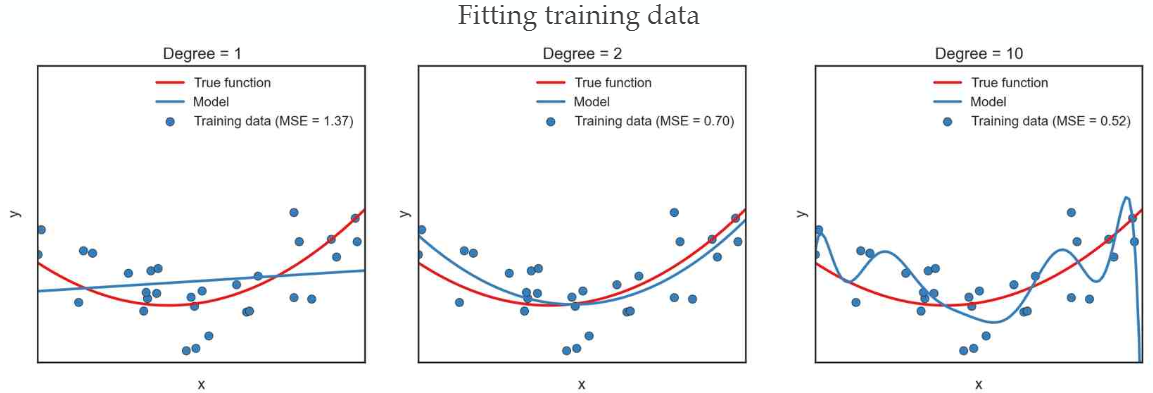
\includegraphics[scale=.3]{gfx/overfitting.png}
	\caption{Fen\'omeno de sobreajuste en polinomios de alto grado}
\end{figure}


Dicho esto, la brecha entre el riesgo emp\'irico y el riesgo esperado puede ser mayor para un conjunto de polinomios de alto grado ya que su alta capacidad les permite sobreajustar un conjunto dado de datos de entrenamiento. (Ver \ref{gfx: overfitting})

Matem\'aticamente, con la capacidad de medici\'on de la dimensi\'on VC, se puede establecer uno de los resultados m\'as importantes en Machine Learning


\begin{proposition}[Cota en la complejidad algoritmica de la estimaci\'on riesgo]
	Sea $d_{ \mathcal{H} }$ la dimensi\'on VC de $\mathcal{H}$ una familia de funciones generalizadora, luego se tiene una probabilidad de al menos $1 - \eta$ que:

\begin{equation}
\label{eq: Cota complejidad algoritmica para distancia de riesgos}
\sup\limits_{h \in \mathcal{H}} {\abs{R(h) - R_n(h)}} \leq \mathcal{O} \left( \sqrt{\frac{1}{2n} \log \left(\frac{2}{\eta}\right) + \frac{d_{\mathcal{H}}}{n} \log \left( \frac{n}{d_{\mathcal{H}}} \right) } \right)
\end{equation}

\end{proposition}

Este l\'imite proporciona una imagen m\'as precisa de la dependencia de la brecha en la elecci\'on de $\mathcal{H}$. Por ejemplo, muestra que para una $d_{ \mathcal{H} }$ fija, se obtiene una convergencia uniforme aumentando el n\'umero de puntos de entrenamiento $n$. Sin embargo, tambi\'en muestra que, para una $n$ fija, la brecha puede ensancharse si aumento $d_{ \mathcal{H} }$. De hecho, para mantener la misma brecha, se debe aumentar $n$ a la misma tasa si $d_{ \mathcal{H} }$ se incrementa. La convergencia uniforme incorporada en este resultado es crucial en el machine learning, ya que uno quiere asegurarse de que el sistema de predicci\'on funciona bien con cualquier dato que se le proporcione. 


Curiosamente, una cantidad que no ingresa en (\ref{eq: Cota complejidad algoritmica para distancia de riesgos}) es el n\'umero de par\'ametros que distinguen a una funci\'on miembro particular $h$ de la familia $\mathcal{H}$. En algunos entornos, como la regresi\'on log\'istica, este n\'umero es esencialmente el mismo que $d_{ \mathcal{H} }$, lo que podr\'ia sugerir que la tarea de optimizar sobre $h \in \mathcal{H} $ es m\'as engorrosa a medida que $d_{ \mathcal{H} }$ aumenta. Sin embargo, este no es siempre el caso. Ciertas familias de funciones son m\'as amenas para minimizar a pesar de tener un n\'umero muy grande o incluso infinito de par\'ametros; en \cite{vapnik:1998} se dise\~naron para aprovechar este hecho [Ver Teorema 10.3].

En general, mientras que los l\'imites tales como (\ref{eq: Cota complejidad algoritmica para distancia de riesgos}) son te\'oricamente interesantes y proporcionan una visi\'on \'util, raramente se usan directamente en la pr\'actica ya que generalmente es m\'as f\'acil estimar la brecha entre riesgo emp\'irico y riesgo esperado con experimentos de \textit{validaci\'on cruzada}. Ahora presentaremos ideas subyacentes a un marco pr\'actico que respeta las concesiones mencionadas anteriormente.

\subsection{Minimizaci\'on de riesgos estructurales}

Un enfoque para elegir una funci\'on de predicci\'on que ha demostrado ser ampliamente exitosa en la pr\'actica es la \textit{minimizaci\'on del riesgo estructural} \cite{vapnik:1974}, \cite{vapnik:1998}. En lugar de elegir una familia gen\'erica de funciones de predicci\'on, sobre las cuales ser\'ia dif\'icil optimizar y estimar la brecha entre los riesgos emp\'iricos y los esperados, se elige una \textit{estructura}, es decir, una colecci\'on de familias de funciones anidadas. Por ejemplo, dicha estructura se puede formar como una colecci\'on de subconjuntos de una determinada familia $\mathcal{H}$ de la siguiente manera: dada una funci\'on de preferencia $\Omega$, elegir varios valores de un \textit{hiperpar\'ametro} $C$, de acuerdo con cada uno de los cuales se obtiene el subconjunto $\mathcal{H}_C := \left\lbrace h \in \mathcal{H} : \Omega (h) \leq C \right\rbrace$. Dado un n\'umero fijo de ejemplos, el aumento de $C$ reduce el riesgo emp\'irico (es decir, el m\'inimo de $R_n (h) $ sobre $h \in \mathcal{H}_C$), pero, despu\'es de cierto punto, t\'ipicamente aumenta la brecha entre los riesgos esperado y emp\'irico. Este fen\'omeno se ilustra en la Figura \ref{gfx: hiperparametros}.


Otras formas de introducir estructuras son considerar un riesgo emp\'irico regularizado $R_n (h) + \lambda \Omega (h)$  que puede verse como el Lagrangiano para minimizar $R_n (h)$ sujeto a $\Omega (h) \leq C$).

\begin{figure}[h]
	\label{gfx: hiperparametros}
	\centering
	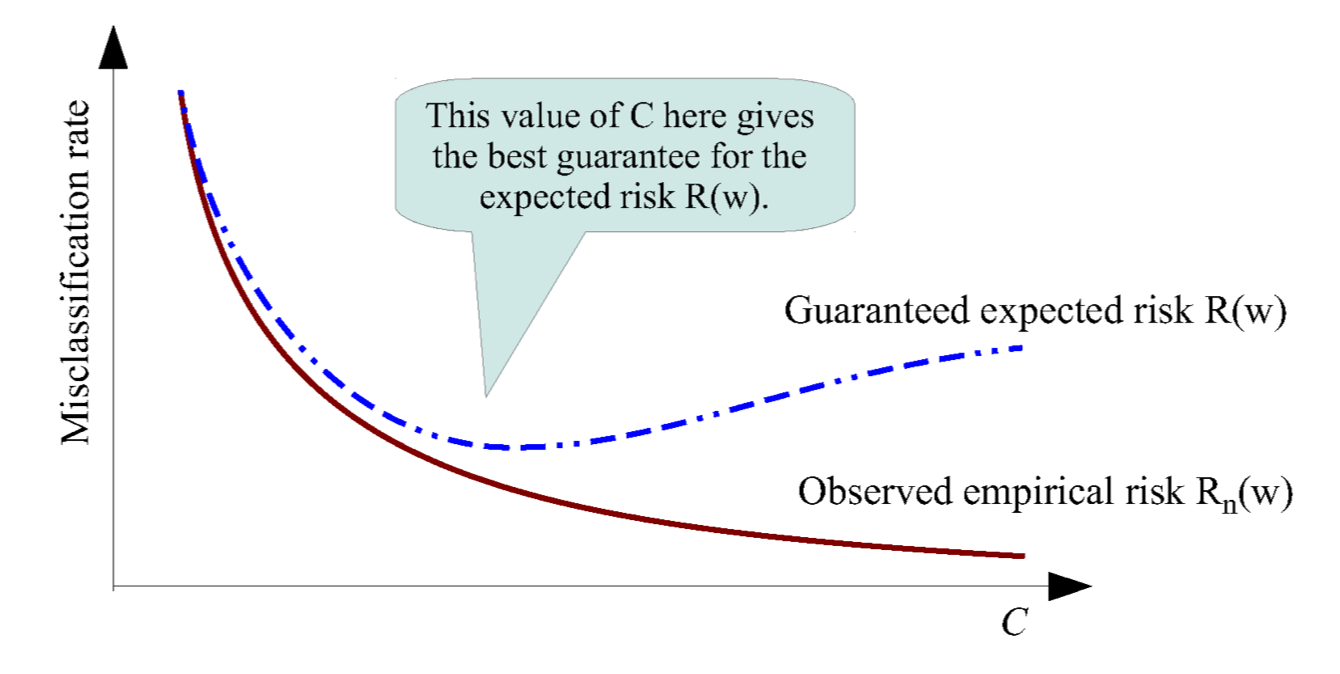
\includegraphics[scale=.3]{gfx/hyperparametros.png}
	\caption{Fen\'omeno de distancia de los riesgos en funcion de la evoluci\'on de hiperpar\'ametros}
\end{figure}

Dada tal configuraci\'on, uno puede evitar estimar la brecha entre el riesgo emp\'irico y esperado dividiendo los datos disponibles en subconjuntos: un \textit{conjunto de entrenamiento} utilizado para producir un subconjunto de soluciones candidatas, un \textit{conjunto de validaci\'on} utilizado para estimar el riesgo esperado para cada candidato, y un \textit{conjunto de prueba} utilizado para estimar el riesgo esperado para el candidato que finalmente se elige. Espec\'ificamente, sobre el conjunto de entrenamiento, uno minimiza una medida de riesgo emp\'irico $R_n$ sobre $\mathcal{H}_C$ para varios valores de $C$. Esto da como resultado un pu\~nado de funciones candidatas. El conjunto de validaci\'on se usa para estimar el riesgo esperado correspondiente a cada soluci\'on candidata, luego de lo cual se elige la funci\'on que arroje el menor valor de riesgo estimado. Suponiendo que se ha utilizado un rango suficientemente grande para $C$, a menudo se encuentra que la mejor soluci\'on no corresponde al mayor valor de $C$ considerado; nuevamente, vea la Figura \ref{gfx: hiperparametros}.


Otro camino, aunque indirecto, hacia la minimizaci\'on del riesgo es emplear un algoritmo para minimizar $R_n$, pero terminar el algoritmo \textit{antes} de que se encuentre un minimizador real de $R_n$. De esta manera, el papel del hiperpar\'ametro lo asume el tiempo de entrenamiento permitido, seg\'un el cual uno encuentra t\'ipicamente las relaciones ilustradas en la Figura \ref{gfx: stopping}. Los an\'alisis te\'oricos relacionados con la idea de la detenci\'on temprana son mucho m\'as desafiantes que los de otras formas de minimizaci\'on del riesgo estructural. Sin embargo, vale la pena mencionar estos efectos ya que la detenci\'on temprana es una t\'ecnica popular en la pr\'actica y, a menudo, es \textit{esencial} debido a las limitaciones del presupuesto computacional.


\begin{figure}[h]
	\label{gfx: stopping}
	\centering
	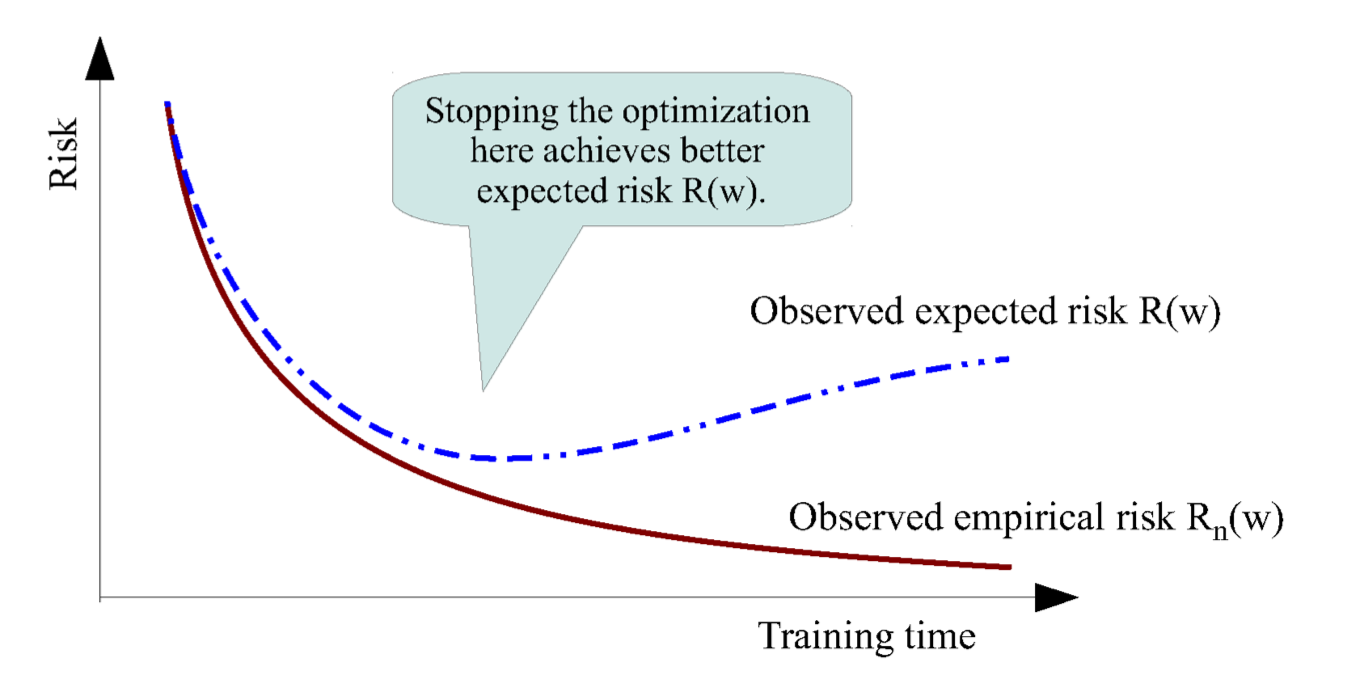
\includegraphics[scale=.3]{gfx/stopping.png}
	\caption{Ilustraci\'on de la detenci\'on temprana. Detener prematuramente la optimizaci\'on del riesgo emp\'irico $R_n$ a menudo resulta en un mejor riesgo esperado $R$. De esta manera, el tiempo de parada juega un papel similar al del hiperpar\'ametro C en la ilustraci\'on de minimizaci\'on de riesgo estructural}
\end{figure}


En general, el principio de minimizaci\'on del riesgo estructural ha demostrado ser \'util para muchas aplicaciones. En lugar de codificar el conocimiento como reglas formales de clasificaci\'on, uno lo codifica mediante preferencias para ciertas funciones de predicci\'on sobre otras, luego explora el rendimiento de varias funciones de predicci\'on que se han optimizado bajo la influencia de dichas preferencias.

\section{Enunciados de problemas de optimizaci\'on formal}

Los problemas de optimizaci\'on en el machine learning surgen a trav\'es de la definici\'on de las funciones de predicci\'on y p\'erdida que aparecen en las mediciones de riesgo esperado y emp\'irico que se pretenden minimizar. Nuestras discusiones giran en torno a las siguientes definiciones.

\subsection{Funciones de Predicci\'on y P\'erdida}
En lugar de considerar un problema de optimizaci\'on variacional sobre una familia gen\'erica de funciones de predicci\'on, suponemos que la funci\'on de predicci\'on $h$ tiene una forma fija y est\'a parametrizada por un vector real $w \in \mathbb{R}^d $ d sobre el cual se realizar\'a la optimizaci\'on. Formalmente, para algunos $h(\cdot ; \cdot): \mathbb{R}^{d_x} \times \mathbb{R}^d \rightarrow \mathbb{R}^{d_y}$ dados y, considerandos la familia de funciones de predicci\'on

\begin{equation}
\mathcal{H} := \lbrace h(\cdot ; w): w \in \mathbb{R}^d \rbrace
\end{equation}

Nuestro objetivo es encontrar la funci\'on de predicci\'on en esta familia que minimice las p\'erdidas incurridas por predicciones inexactas. Para este prop\'osito, asumimos una funci\'on de p\'erdida dada $ \ell : \mathbb{R}^{d_y} \times \mathbb{R}^{d_y} \rightarrow \mathbb{R}$ como aquella que, dado un par de entrada-salida $(x, y)$, produce la p\'erdida $ \ell (h(x;w),y)$ cuando $h (x; w)$ e $y$ son las salidas predichas y verdaderas, respectivamente.

\subsection{Riesgo esperado}
Idealmente, el vector de par\'ametros $\omega$ se elige para minimizar la p\'erdida esperada en la que se incurrir\'ia con \textit{cualquier} par de entrada-salida. Para expresar esta idea formalmente, suponemos que las p\'erdidas se miden con respecto a una distribuci\'on de probabilidad $P (x, y)$ que representa la verdadera relaci\'on entre las entradas y las salidas. Es decir, suponemos que el espacio de entrada-salida $\mathbb{R}^{d_x} \times \mathbb{R}^{d_y}$ est\'a dotado con $P: \mathbb{R}^{d_x} \times \mathbb{R}^{d_y} \rightarrow [0,1]$ y la funci\'on objetivo que deseamos minimizar es

\begin{equation}
\label{eq: Riesgo esperado}
R(w) = \int\limits_{\mathbb{R}^{d_x}\times \mathbb{R}^{d_y}} {\ell \left(h(x;w), y\right) dP(x,y)} = \mathbb{E} \left[ \ell \left( h(x;w), y \right) \right]
\end{equation}

Decimos que $R : \mathbb{R}^{d} \rightarrow \mathbb{R}$ produce el \textit{riesgo esperado} (es decir, la p\'erdida esperada) dado un vector de par\'ametro $w$ con una respectiva distribuci\'on de probabilidad $P$.

\subsection{Riesgo emp\'irico}
Si bien puede ser deseable minimizar (\ref{eq: Riesgo esperado}), tal objetivo es insostenible cuando no se cuenta con informaci\'on completa sobre $P$. Por lo tanto, en la pr\'actica, uno busca la soluci\'on de un problema que involucra una estimaci\'on del riesgo esperado $R$. En el aprendizaje supervisado, uno tiene acceso (ya sea de una vez o de manera incremental) a un conjunto de  $n \in \mathbb{N}$ muestras de entrada y salida independientes $\left\lbrace (x_i, y_i) \right\rbrace_{i=1}^{n} \subset \mathbb{R}^{d_x} \times \mathbb{R}^{d_y}$, con las cuales se puede definir la funci\'on de riesgo emp\'irico $R_n : \mathbb{R}^d \rightarrow \mathbb{R}$ dada por la ecuaci\'on 

\begin{equation}
\label{eq: Riesgo empirico}
R_n(\omega) = \frac{1}{n} \sum\limits_{i=1}^{n} {l \left( h(x;w), y\right)}
\end{equation}

En t\'erminos generales, la minimizaci\'on de $R_n$ puede considerarse el problema pr\'actico de optimizaci\'on de inter\'es. Por ahora, consideramos la medida no regularizada (\ref{eq: Riesgo empirico}), pero notemos que los m\'etodos de optimizaci\'on que discutiremos en las secciones siguientes pueden aplicarse f\'acilmente cuando se incluye un t\'ermino suave de regularizaci\'on.

\subsection{Notaci\'on simplificada}
Las expresiones (\ref{eq: Riesgo empirico}) y (\ref{eq: Riesgo esperado}) muestran expl\'icitamente c\'omo los riesgos esperado y emp\'irico dependen de la funci\'on de p\'erdida, espacio de muestra o conjunto de muestras, etc. Sin embargo, cuando hablamos de m\'etodos de optimizaci\'on, a menudo emplearemos una notaci\'on simplificada que tambi\'en ofrece algunos caminos para generalizar ciertas ideas algor\'itmicas. En particular, representemos una muestra (o conjunto de muestras) por una variable aleatoria $\upxi$; por ejemplo, uno puede imaginar una realizaci\'on de $\upxi$ como una muestra \'unica $(x, y)$ de $\mathbb{R}^{d_x} \times \mathbb{R}^{d_y}$, o una realizaci\'on de $\upxi$ podr\'ia ser un conjunto de muestras $\left\lbrace(x_i, y_i)\right\rbrace_{i \in S}$. Adem\'as, podemos referirnos a la p\'erdida incurrida para un dado $(w, \upxi)$ como $g (w; \upxi )$, es decir, $g$ es la composici\'on de la funci\'on de p\'erdida y la funci\'on de predicci\'on $h$.

De esta manera, el riesgo esperado para una $w$ dada es el valor esperado de esta funci\'on compuesta tomada con respecto a la distribuci\'on de $\upxi$:

\begin{equation}
\label{Riesgo esperado 3}
R(w) = \mathbb{E} \left [ g(w; \upxi) \right ]
\end{equation}

De manera similar, dado un conjunto de realizaciones $\left\lbrace \upxi_{\left [ i \right ]} \right\rbrace _{i=1}^{n}$ de $\upxi$ correspondientes a un conjunto de muestras $\left\lbrace (x_i, y_i) \right\rbrace_{i=1}^{n}$, definamos la p\'erdida incurrida por el vector de par\'ametro $w$ con respecto a la i-\'esima muestra como

\begin{equation}
\label{funci\'on p\'erdida de w}
g_i (w) := g(w, \upxi_{\left [ i \right ]})
\end{equation}

y luego escribamos el riesgo emp\'irico como el promedio de las p\'erdidas de la muestra:

\begin{equation}
\label{Riesgo empirico 3}
R_n(w) = \frac{1}{n}\sum\limits_{i=1}^{n} g_i (w)
\end{equation}

Para referencia futura, usamos $\upxi_{\left [ i \right ]}$ para denotar el i-\'esimo elemento de un conjunto fijo de realizaciones de una variable aleatoria $\upxi$, mientras que, comenzando en la parte \ref{pt:algoritmosestocasticos}, utilizaremos $\upxi_{\left [ k \right ]}$ para denotar el k-\'esimo elemento de una secuencia de variables aleatorias .

\subsection{M\'etodos Estoc\'asticos vs. Optimizaci\'on por Batch}
Ahora vamos a introducir algunos algoritmos de optimizaci\'on fundamentales para minimizar el riesgo. Por el momento, dado que es la configuraci\'on t\'ipica en la pr\'actica, presentamos dos clases de algoritmo en el contexto de minimizar el riesgo emp\'irico medido $R_n$ en (\ref{Riesgo empirico 3}). Hay que tener en cuenta, sin embargo, que gran parte de nuestra discusi\'on posterior se centrar\'a en el rendimiento de los algoritmos al considerar la verdadera medida de inter\'es, es decir, el riesgo esperado $R$ en (\ref{Riesgo esperado 3}).

Los m\'etodos de optimizaci\'on para el machine learning se dividen en dos grandes categor\'ias. Nos referimos a ellos como estoc\'asticos y por Batch. El m\'etodo protot\'ipico de optimizaci\'on estoc\'astica es el m\'etodo del gradiente estoc\'astico (DE) \cite{robbins:1951}, que, en el contexto de minimizar $R_n$ y con $w_1\in \mathbb{R}^d$ dado, se define por
\begin{equation}
\label{def: DE}
w_{k+1} \gets w_k - \alpha_k \nabla g_{i_k} (w_k)
\end{equation}

Aqu\'i, para todo $k \in \mathbb{N} := \left\lbrace 1, 2, ... \right\rbrace $, el \'indice $i_k$ (correspondiente a la variable aleatoria $\upxi_{\left[ i_k \right]}$, es decir, el par de muestras $(x_{i_k}, y_{i_k})$) se elige \textit{al azar} de $\left\lbrace 1,. . . , n \right\rbrace$ y $\alpha _k$ es un incremento positivo. Cada iteraci\'on de este m\'etodo es, por lo tanto, muy barata, y solo incluye el c\'alculo del gradiente $\nabla g_{i_k} (w_k)$ correspondiente a una muestra. El m\'etodo es notable porque la secuencia de iteraci\'on no est\'a determinada \'unicamente por el
	la funci\'on $R_n$, el punto de inicio $w_1$, y la secuencia de incrementos $\left\lbrace \alpha _k \right\rbrace $, como lo har\'ia en un algoritmo de optimizaci\'on determinista. Por el contrario, $\left\lbrace w_k \right\rbrace $ es un proceso estoc\'astico cuyo comportamiento est\'a determinado por la secuencia aleatoria $\left\lbrace i_k \right\rbrace $. A\'un as\'i, como veremos en nuestro an\'alisis en el cap\'itulo \ref{ch:convergenciaL1}, mientras que cada direcci\'on $- \nabla g_{i_k} (w_k)$ podr\'ia no ser una de descendencia de $w_k$ (en el sentido de producir una derivada direccional negativa para $R_n$ de $w_k$), s\'i es una direcci\'on de descenso \textit{en esperanza}, luego la secuencia $\left\lbrace w_k \right\rbrace $ puede guiarse hacia un minimizador de $R_n$.
	
	Para muchos en la comunidad de investigaci\'on de optimizaci\'on, un enfoque por \textit{Batch} es una idea m\'as natural y conocida. El m\'etodo m\'as simple de esta clase es el algoritmo de descenso m\'as pronunciado -tambi\'en conocido como gradiente, descenso de gradiente por Batch o m\'etodo de gradiente completo- (GD)que se define mediante la siguiente iteraci\'on:
	
	\begin{equation}
	\label{gradiente de Batch}
	w_{k+1} \gets w_k - \alpha_k \nabla R_n(w_k) = w_k -\frac{\alpha_k}{n} \sum\limits_{i=1}^{n} {\nabla g_i (w_k)}
	\end{equation}
	
	Calcular el paso $- \alpha_k \nabla R_n (w_k)$ en tal enfoque es m\'as costoso que calcular el paso $- \alpha_k \nabla g_{i_k} (w_k)$ en DE, aunque se puede esperar que se calcule un mejor paso cuando todas las muestras se consideran en una iteraci\'on.
	
	Los enfoques estoc\'astico y por Batch ofrecen diferentes compensaciones en t\'erminos de costos de iteraci\'on y mejora esperada de la iteraci\'on para minimizar el riesgo emp\'irico. ¿Por qu\'e, entonces, DE ha alcanzado tal prominencia en el contexto del machine learning a gran escala? Comprender el razonamiento detr\'as de esto requiere una consideraci\'on cuidadosa de las compensaciones computacionales entre los m\'etodos estoc\'astico y por Batch, as\'i como una mirada m\'as profunda en sus habilidades para garantizar la mejora en el subyacente riesgo esperado $R$. Comenzaremos a investigar estos temas en la siguiente subsecci\'on.
	
	\section{Motivaci\'on para los m\'etodos estoc\'asticos}
	Antes de analizar las fortalezas de los m\'etodos estoc\'asticos, como DE, no se debe perder de vista el hecho de que los enfoques por Batch poseen algunas ventajas intr\'insecas. Primero, cuando uno ha reducido el problema estoc\'astico de minimizar el riesgo esperado $R$ para enfocarse exclusivamente en el problema determinista de minimizar el riesgo emp\'irico $R_n$, el uso de informaci\'on de gradiente completo en cada iteraci\'on abre la puerta para muchos m\'etodos de optimizaci\'on determin\'isticos basados en gradiente. Es decir, en un enfoque por Batch, uno tiene a su disposici\'on la gran cantidad de t\'ecnicas de optimizaci\'on no lineal que se han desarrollado en las \'ultimas d\'ecadas, incluido el m\'etodo de gradiente completo o gradiente de Batch (\ref{gradiente de Batch}), pero tambi\'en gradiente acelerado, gradiente conjugado, cuasi-Newton y m\'etodos inexactos de Newton \cite{nocedal:2006}. Segundo, debido a la estructura de suma de $R_n$, un m\'etodo por Batch puede beneficiarse f\'acilmente de la paralelizaci\'on ya que la mayor parte del c\'alculo se basa en evaluaciones de $R_n$ y $\nabla R_n$. Los c\'alculos de estas cantidades pueden incluso realizarse de forma distribuida.
	
	A pesar de estas ventajas, existen razones intuitivas, pr\'acticas y te\'oricas para seguir un enfoque estoc\'astico. Perm\'itanos motivarlos contrastando la iteraci\'on DE caracter\'istica (\ref{def: DE}) con la iteraci\'on de gradiente de Batch completo (\ref{gradiente de Batch}).

\section{Organizaci\'on de la Tesis}

Esta Tesis esta organizada seg\'un la categorizaci\'on mas est\'andar de los algoritmos encontrados en Machine Learning.

La primer parte (\ref{pt:introduccion}) refiere a la motivaci\'on tanto matem\'atica como algoritmica y del \'area para analizar la convergencia de los algoritmos presentados, como a su vez los contenidos preliminares usados a lo largo del documento.

La segunda parte (\ref{pt:algoritmosbatch}) trata exclusivamente los algoritmos deterministicos, comunmente denominados de \textit{tipo batch}. En el Cap\'itulo \ref{ch:convergenciaPuntual} , utilizando la gran referencia \cite{nesterov:2004}, analizamos la convergencia puntual del descenso de gradiente con condiciones de convexidad d\'ebil y luego la convergencia \textit{lineal} con convexidad mas fuerte. Luego en el cap\'itulo \ref{ch:teorema-de-variedad-estable} nos basamos en \cite{lee:2017} para ver a estos algoritmos como discretizaciones de sistemas din\'amicos y con elt eorema de la variedad estable conclu\'imos un m\'etodo pr\'actico para analizar la convergencia \textit{casi todo punto}; esta forma de analizar los algortitmos es aplicada en el cap\'itulo \ref{ch: aplicaciones} con varios algoritmos est\'andar en el \'area. Finalmente en el cap\'itulo \ref{ch:resultadosNegativos} nos basamos en \cite{du:2017} para ver que aunque se tiene convergencia \textit{casi todo punto}, la complijdad algoritmica del descenso de gradiente es exponencial.

Esto nos motiva pasar a analizar los algoritmos estoc\'asticos en la parte \ref{pt:algoritmosestocasticos}, donde nos basamos en \cite{bottou:1999} y \cite{bottou:2016} para analizar en el cap\'itulo \ref{ch:convergenciaL1} la convergencia en \textit{norma $L1$} al m\'inimo (o a un entorno de \'este) y finalmente en el cap\'itulo \ref{ch:convergenciaCTP} la convergencia \textit{casi todo punto} tanto en los casos convexo como no convexo, ya que el algoritmo induce un proceso estoc\'astico que induce una \textit{cuasi-martingala} convergente.

\smallskip
